\begin{frame}
    \frametitle{未向世界銀行申報的債務}


    \begin{itemize}
        \item 接收機關大量包含國有企業與特設機構:鮮少為低所得國家內入統計
        \item 使用世界銀行 Debtor Reporting System (DRS),取得各國向中國借貸金額\footnotemark{}
        \item 與 \citet*{Horn-Reinhart-Trebesch-21} 所計算出來的做比較
    \end{itemize}

    \footnotetext{這裡指的是承付貸款 (loan commitments)而非撥付金額 (disbursement)。換句話說看的是總共承諾要償還的,不是當期要償還的金額。 \citet*{Horn-Reinhart-Trebesch-21}中提此為機密資料。}

\end{frame}

\begin{frame}
    \frametitle{隱匿債務統計}

    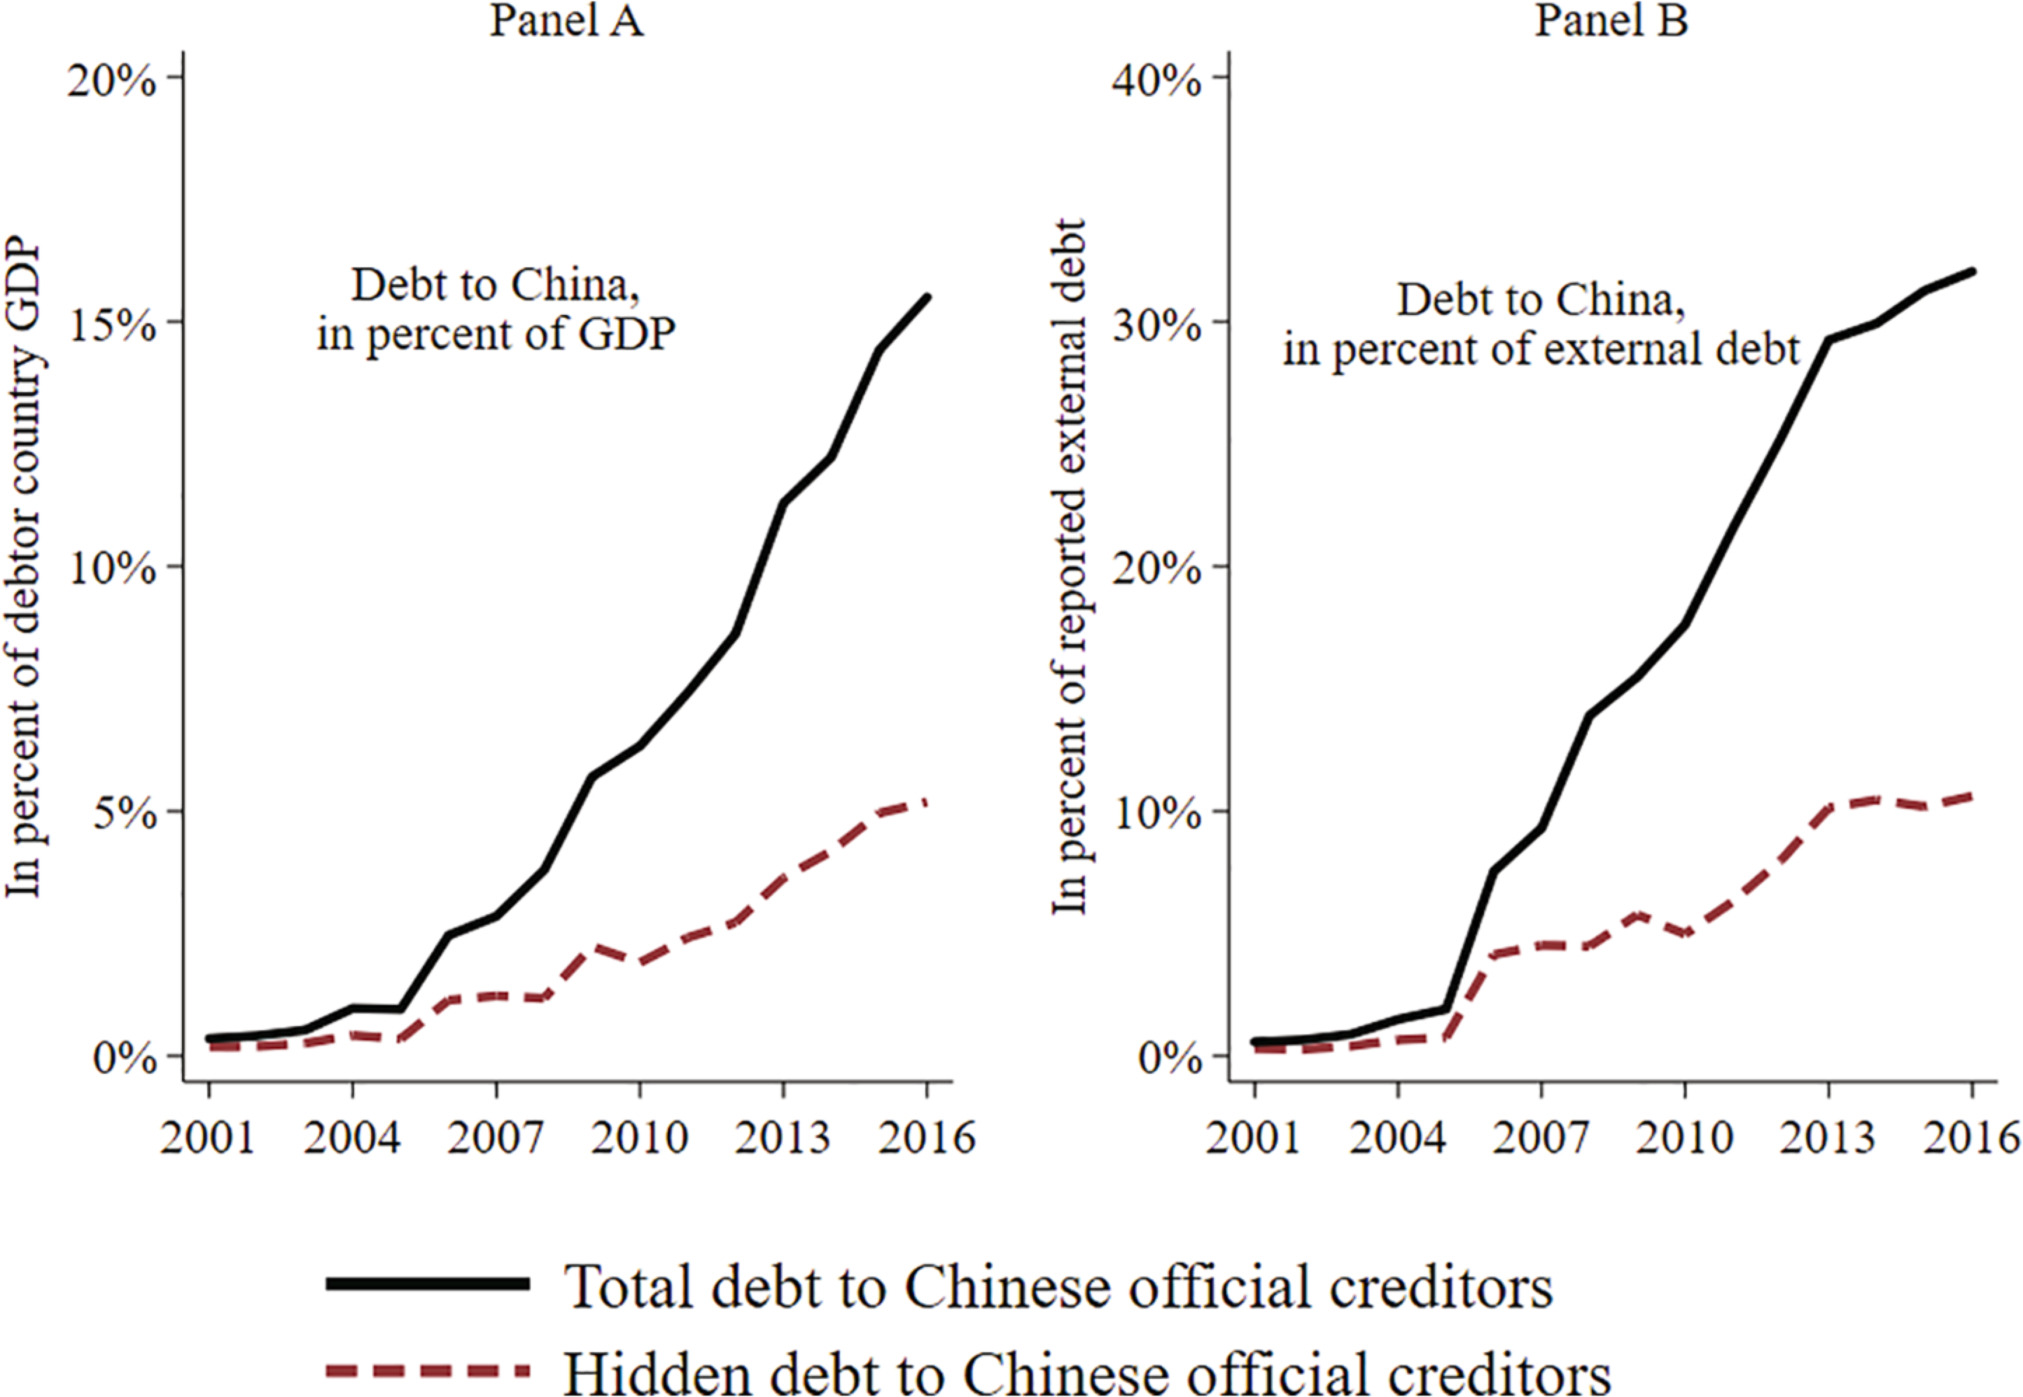
\includegraphics[width = \textwidth]{fig/fig12.jpg}

\end{frame}

\begin{frame}
將樣本國家控制在前50被影響國家中
\begin{itemize}
    \item 中國債務佔 15\% GDP
    \item 有 5\% 中國債務佔 GDP 的比重,未被統計在世界銀行的資料庫中
    \item 以總外債來看,有 10\% 的隱匿債務
\end{itemize}

\end{frame}

\begin{frame}
    \frametitle{貨幣互換債務}

    還有一部分的隱匿債務來自於中國央行與其他國家之間在央行的貨幣互換 (swap line) \citep*{Bahaj-Saleem}。
    \begin{block}{Swap Line}
        央行之間簽訂的一種協議,當金融危機發生時,央行可以通過這種協議來獲取對方央行的貨幣,以維持本國貨幣的穩定。
    \end{block}

    \begin{itemize}
        \item PBoC的貨幣互換借款期限通常很短(3至6個月)
        \item 中國似乎多次延長到三年,實際期限類似於長期債務
        \item 世界銀行認為貨幣互換債務應該被視為中國直接(不可轉讓)、長期的債務工具
        \item 自2009年以來,PBoC已與38個中央銀行建立了雙邊貨幣互換安排,總額超過5000億美元,是全球最大的貨幣互換網絡之一
    \end{itemize}

\end{frame}